%&"..\virtual"

\begin{document}
    \title{DPDK}
    \maketitle
    \tableofcontents
    \section{要求}

    DPDK performance test:

    \begin{enumerate}[(1)]
        \item Create two virtual machines on KVM.
        \item Compile and install DPDK library on each virtual machine.
        \item Compile and run DPDK sample application l2fwd on VM2, then compile and run pktgen-dpdk on VM1.  pkgen-dpdk will record the size of the packages VM1 sends and the amount of packages received from VM2,  while l2fwd just send back the packages it received from VM1.
        \item Evaluate DPDK's performance of L2 forwarding.
    \end{enumerate}

    \section{编译安装 DPDK}

    按照官方文档\cite{dpdk}编译 DPDK,如图 \ref{fig:meson} 和 \ref{fig:ninja} 所示。

    \code[language=bash]{INSTALL.sh}

    \begin{figure}[H]
        \centering
        \begin{minipage}{0.48\textwidth}
            \centering
            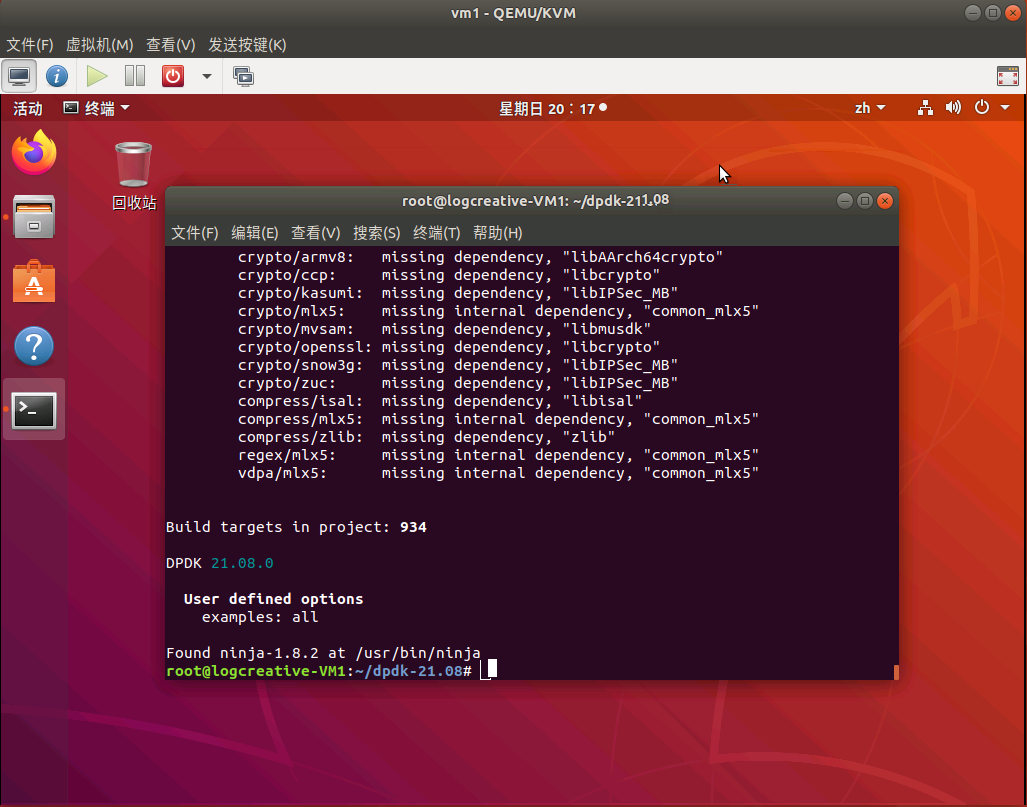
\includegraphics[width=\linewidth]{meson}
            \caption{meson 配置}\label{fig:meson}
        \end{minipage}
        \begin{minipage}{0.48\textwidth}
            \centering
            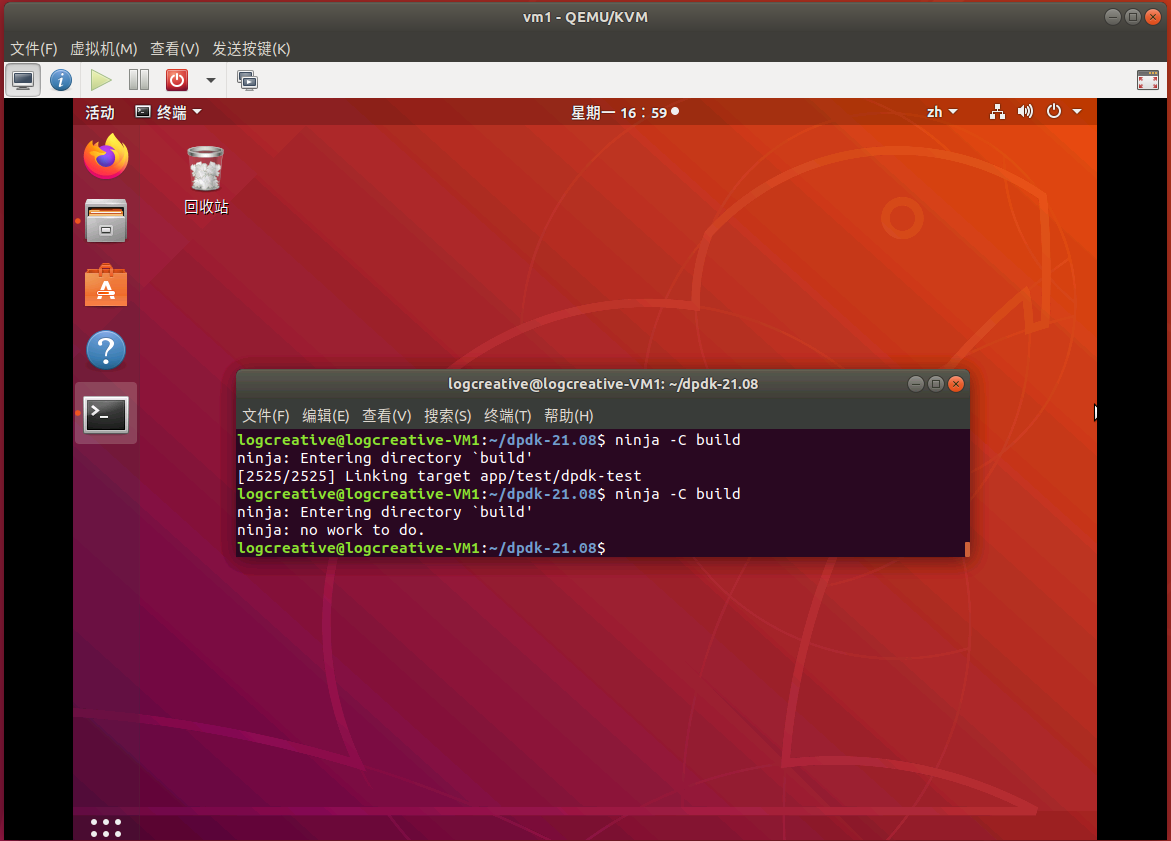
\includegraphics[width=\linewidth]{ninja}
            \caption{ninja 编译}\label{fig:ninja}
        \end{minipage}
    \end{figure}

    之后对该虚拟机进行克隆,得到另一个已经安装 DPDK 的虚拟机。

    \bibliography{ref}

\end{document}